\newpage
\clearpage

\section{Redes Neurais Convolucionais}
\label{cnn}

Dentre os diversos tipos de redes de aprendizado profundo, as mais amplamente utilizadas atualmente para lidar com visão computacional, processamento de imagens e possuindo um valor notável para o trabalho com dados espaciais \citep{Goodfellow2016, ponti2018funciona, Ghosh2019}, destacam-se as \textit{Convolutional Neural Networks} (CNNs) \citep{LeCun1999}. As CNNs recebem esse nome por empregarem camadas convolucionais, sendo especialmente proeminentes e eficazes nesses contextos.

É inegável que as CNNs são consideradas o estado-da-arte em várias competições \citep{Parkhi2015}, além de serem modelos bioinspirados de sucesso \citep{Goodfellow2016}. Elas são capazes de simular pontos cerebrais responsáveis pela interpretação de impulsos visuais, reproduzindo propriedades do córtex visual. Além disso, essas redes têm a capacidade de extrair diferentes características, utilizando a combinação das camadas de convolução (Seção \ref{cnn:conv}) juntamente com operações de \textit{pooling} que tem o papel de compressão e serão detalhadas na Seção \ref{cnn:pooling}.

Entre a vasta gama de arquiteturas disponíveis para as CNNs, destacam-se algumas das mais influentes: AlexNet \citep{krizhevsky2012imagenet}, VGGNet \citep{Simonyan2015}, ResNet \citep{He2016}, GoogLeNet \citep{Szegedy2015}, MobileNet \citep{Howard2017} e DenseNet \citep{Huang2017}. Essas arquiteturas possuem contribuições significativas e têm sido aplicadas em uma variedade de contextos, cada uma com suas características e aplicações específicas.

Um modelo indicando uma entrada, as camadas convolucionais iniciais e finais, que são utilizadas para extração de atributos, bem como o sistema de \textit{pooling} e a camada de saída (ou camada densa) são representados por meio da Figura \ref{cnn:fig:10}.

\begin{figure}[H]
    \centering
    \caption{Modelo de CNN.}
    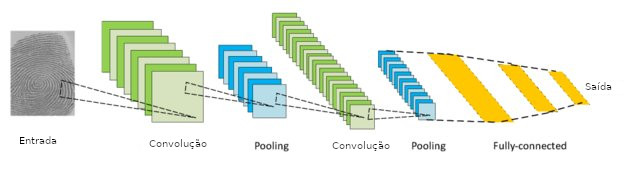
\includegraphics[width=1\linewidth]{recursos/imagens/deep/cnn.jpg}
    \label{cnn:fig:10}

    Fonte: retirada e adaptado de \cite{Minaee2021DeepClassification}.
\end{figure}

Dessa forma, nas seções seguintes, os elementos fundamentais que compõem uma rede neural convolucional serão minuciosamente explorados. Estes incluem a camada convolucional (Seção \ref{cnn:conv}), a camada de \textit{pooling} (Seção \ref{cnn:pooling}), o componente \textit{dropout} (Seção \ref{cnn:dropout}) e a camada de saída (Seção \ref{cnn:output}) da rede. Adicionalmente, serão abordados temas complementares que impactam significativamente no desempenho das CNNs, tais como transferência de aprendizado (Seção \ref{cnn:transfer}) e aumento de dados (Seção \ref{cnn:augment}). Por fim, será explorada uma das arquiteturas que exerceu considerável influência na evolução desse campo, a VGG (Seção \ref{cnn:vgg}).


\subsection{Camada Convolucional}
\label{cnn:conv}

Na arquitetura das CNNs, a modelagem de cada neurônio presente na camada convolucional envolve a aplicação de um filtro na imagem em análise \citep{ponti2018funciona}. Esses filtros são compostos por pesos e a operação de convolução é categorizada como uma operação linear \citep{Goodfellow2016}, resultando nos chamados mapas de características (\textit{feature maps}, em inglês).

É fundamental destacar que entre as camadas convolucionais existem $N$ filtros, cujos parâmetros são definidos de acordo com a natureza do problema em questão, utilizando seus resultados para formar tensores, conforme comentado por \cite{ponti2018funciona}.

A operação de convolução pode ser ilustrada pela Figura \ref{cnn:fig:6}, onde uma imagem de entrada é representada pela matriz de maior escala. Nesse processo, utiliza-se uma janela, conhecida como \textit{kernel}, composta por pesos, que convolui com a matriz de entrada para extrair características específicas da imagem, mantendo a integridade das informações sobre sua disposição espacial.

Essas operações são fundamentais nas CNNs, pois permitem a extração eficiente de características importantes das imagens, o que é crucial para a eficácia e a precisão do processo de aprendizado da rede neural convolucional.

\begin{figure}[H]
    \centering
    \caption{Representação do processo de convolução.}
    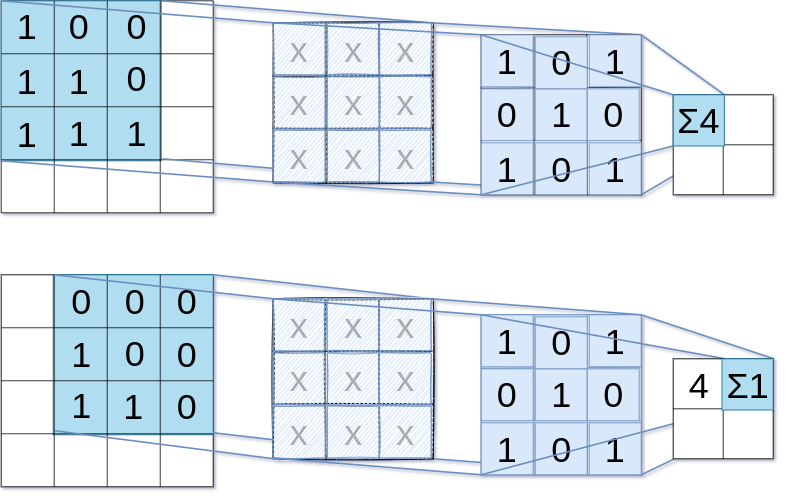
\includegraphics[width=1\linewidth]{recursos/imagens/deep/2d_convolution.png}
    \label{cnn:fig:6}

    Fonte: do próprio autor.
\end{figure}

Ainda na Figura \ref{cnn:fig:6}, é possível observar o processo de deslizamento do \textit{kernel} durante a operação de convolução, resultando em um dos valores presentes na saída. Esse processo é repetido até que toda a imagem seja percorrida, de maneira sequencial da esquerda para a direita e de cima para baixo, movimentando-se através das linhas e colunas.

O processo iterativo de aplicação da máscara sobre a imagem pode ser representado matematicamente pela Equação \ref{cnn:eq:conv} \citep{Gonzalez2009}:

\begin{equation}
    \label{cnn:eq:conv}
    w(x,y)*f(x,y) = \sum\limits_{s=-a}^a \sum\limits_{t=-b}^b w(s,t)f(x-s,y-t),
\end{equation}
onde $x$ e $y$ representam coordenadas espaciais da matriz de entrada, $w(x,y)$ é o valor do \textit{pixel} na posição $(x,y)$ da janela e $f(x,y)$ é o valor do \textit{pixel} na posição $(x,y)$ da matriz de entrada. Além disso, vale citar que $s$ e $t$, representam variáveis de iteração usadas para percorrer a máscara e, $m$ e $n$ representam as dimensões da máscara, utilizadas para definir os limites de iteração nas somas duplas $a$ e $b$, conforme especificado pelas Equações \ref{cnn:eq:row} e \ref{cnn:eq:col} \citep{Gonzalez2009}:

\begin{equation} 
   \label{cnn:eq:row}
   a = (m-1)/2,
\end{equation}

\begin{equation} 
   \label{cnn:eq:col}
   b = (n-1)/2.
\end{equation}

É crucial ressaltar que a convolução é um processo de média móvel, isto é, implica no cálculo da média ponderada de uma janela específica na imagem, correspondente ao tamanho do \textit{kernel} utilizado. Nesse contexto, o \textit{kernel} define os pesos aplicados aos pontos da janela. Consequentemente, à medida que o \textit{kernel} desliza pela imagem, novas janelas são definidas e suas médias ponderadas são computadas.

Essa abordagem de convolução, com seu deslizamento e cálculo ponderado, é essencial para a extração de informações significativas da imagem, contribuindo para a identificação de padrões relevantes ao longo do processo de aprendizado da rede neural convolucional.


\subsection{Camada de \textit{Pooling}}
\label{cnn:pooling}

Dentro do contexto das camadas de \textit{pooling}, é relevante mencionar que essas camadas são amplamente empregadas nas CNNs com o propósito de reduzir o tempo de treinamento, já que sua função primária é diminuir a dimensionalidade dos mapas de características entre as iterações da rede.

É digno de nota que a adaptação e evolução desses métodos de \textit{pooling} têm recebido crescente atenção na literatura recente \citep{Sabri2020AClassificationb, Zafar2022ANetworks}. Cada modificação busca contribuir para a solução de problemas específicos, evidenciando o constante desenvolvimento dessas técnicas na área de visão computacional e aprendizado profundo.

Ademais, vale ressaltar que na literatura existem diversos modelos de \textit{pooling} que se destacam no uso em redes de aprendizado profundo. Entre eles, destacam-se o \textit{max pooling}, \textit{average pooling}, \textit{median pooling} e \textit{weighted average} \citep{Goodfellow2016}. Há também outros modelos comumente encontrados em redes mais modernas, como o \textit{global average pooling}, \textit{global max pooling} e \textit{astrous spatial pyramid pooling}, principalmente em aplicações de segmentação ou com propostas alternativas. Alguns desses modelos serão discutidos a seguir.

\subsubsection{\textit{Max Pooling}}
\label{cnn:pooling:max_pooling}
O \textit{max pooling} é uma das técnicas mais conhecidas e amplamente utilizadas para realizar o \textit{pooling} em CNNs \citep{Zafar2022ANetworks, Paul2019DimensionalityPooling}. Esta técnica é preferida devido à sua simplicidade, não exigindo ajuste de parâmetros, além de atender de forma eficiente à necessidade de reduzir a dimensionalidade das entradas \citep{Boureau2010ARecognition}.

O funcionamento do \textit{max pooling}, denotado por $f_{\max}(\boldsymbol{X})$, pode ser representado pela Equação \ref{cnn:eq:pooling:max_pooling}:

\begin{equation}
\label{cnn:eq:pooling:max_pooling}
f_{\max}(\boldsymbol{X})_{i, j, k} = \max_{m, n} X_{i \cdot s_x + m, j \cdot s_{y} + n, k}.
\end{equation}

Nesta equação, $\boldsymbol{X}$ representa o valor de entrada, $(i, j)$ são os índices do valor de saída e $k$ é a quantidade de canais (ou camadas) associadas ao valor de entrada. Além disso, $s_{x}$ e $s_{y}$ representam os tamanhos de deslocamento (ou \textit{stride}) horizontal e vertical, respectivamente. Finalmente, $m$ e $n$ representam as posições dentro da janela de \textit{pooling} ao longo das dimensões horizontal e vertical, respectivamente, sendo que essas variáveis variam de acordo com o tamanho da janela de pooling e o passo (\textit{stride}) ao percorrer a matriz de entrada para realizar a operação de \textit{max pooling}.

O resultado da operação de \textit{max pooling} é obtido utilizando um \textit{kernel} como ilustrado na Figura \ref{cnn:fig:7}, onde a técnica captura apenas os maiores valores do mapa de características.

\begin{figure}[H]
    \centering
    \caption{\textit{Max pooling}.}
    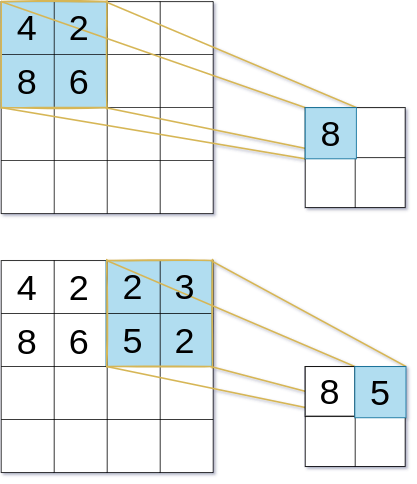
\includegraphics[width=0.5\linewidth]{recursos/imagens/deep/max_pooling.png}
    \label{cnn:fig:7}

    Fonte: do próprio autor.
\end{figure}

É relevante destacar que a aplicação da técnica de \textit{max pooling} adiciona uma leve invariância por translação ao processo. No entanto, de modo geral, isso não afeta de maneira significativa os valores de saída da camada de \textit{pooling} \citep{Boureau2010ARecognition}.

A técnica de \textit{max pooling} é conhecida por preservar características importantes da entrada, ao mesmo tempo em que reduz a dimensionalidade dos mapas de características, tornando-os mais computacionalmente eficientes e facilitando a detecção de padrões por camadas subsequentes da rede neural convolucional. Todavia, essa técnica não se demonstra adequada quando se trata da preservação de informação da entradas \citep{Liu2019Multi-LevelNetworks}, visto que se realiza a redução de dimensionalidade de forma local.

\subsubsection{\textit{Average Pooling}}
\label{cnn:pooling:avg_pooling}
A técnica de \textit{average pooling}, semelhante à técnica de \textit{max pooling} descrita na Seção \ref{cnn:pooling:max_pooling}, é considerada uma técnica estabelecida e tradicional para aplicação em CNNs \citep{Zafar2022ANetworks, Paul2019DimensionalityPooling}. O funcionamento de ambas as técnicas é bastante semelhante, diferenciando-se principalmente pela aplicação da média em vez da função $\max$ para obter o resultado do \textit{Average Pooling}, denotado por $f_{avg}(\boldsymbol{X})$, conforme ilustrado na Equação \ref{cnn:eq:pooling:avg_pooling}:

\begin{equation}
    \label{cnn:eq:pooling:avg_pooling}
    f_{avg}(\boldsymbol{X})_{i, j, k} = \frac{1}{f{x} \cdot f_{y}} \sum_{m, n} X_{i \cdot s_x + m, j \cdot s_{y} + n, k}.
\end{equation}

Nesta equação, $\boldsymbol{X}$ representa o valor de entrada, $(i, j)$ são os índices do valor de saída e $k$ é o número de camadas. Os parâmetros $s_x$ e $s_y$ representam os valores de \textit{stride} vertical e horizontal, respectivamente, enquanto os tamanhos dos filtros $f_x$ e $f_y$ determinam a janela de \textit{pooling}, centrada nos índices de saída $(i,j)$, tendo $m$ e $n$ referentes às posições locais dentro da janela de \textit{pooling}, assim como na Equação \ref{cnn:eq:pooling:max_pooling}. Uma representação visual dessa fórmula é ilustrada na Figura \ref{cnn:fig:avg_pooling}.

\begin{figure}[H]
    \centering
    \caption{\textit{Average pooling}.}
    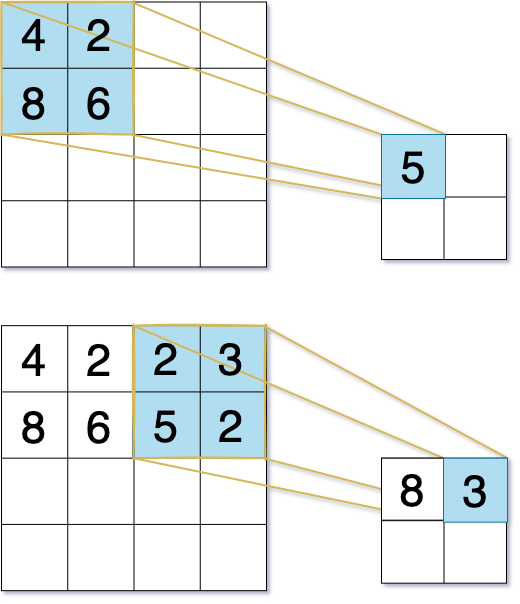
\includegraphics[width=0.5\linewidth]{recursos/imagens/deep/avgpooling.png}
    \label{cnn:fig:avg_pooling}

    Fonte: do próprio autor.
\end{figure}

Por fim, é relevante mencionar que o resultado visual obtido pelo \textit{average pooling} tende a extrair características de maneira mais suave do que o \textit{max pooling}. Enquanto o \textit{max pooling} enfatiza características mais proeminentes, como bordas, o método de \textit{average pooling} tende a extrair características mais suaves, como informações relacionadas às cores. Essa técnica foi utilizada na primeira rede neural profunda baseada em convolução \citep{LeCun1998Gradient-basedRecognition}. Contudo, observam-se desafios semelhantes em relação à preservação da espacialidade das entradas \citep{Liu2019Multi-LevelNetworks}, como ocorre também no algoritmo de \textit{max pooling}.

\subsubsection{\textit{Global Average Pooling}}
\label{cnn:pooling:global_avg_pooling}
A técnica de \textit{Global Average Pooling}, por sua vez, permite a redução dos mapas de características a um único valor por camada, como ilustrado na Figura \ref{cnn:fig:8}.

\begin{figure}[H]
    \centering
    \caption{\textit{Global Average Pooling}.}
    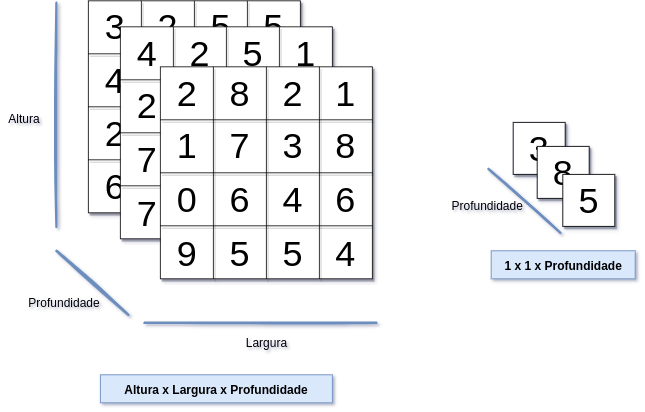
\includegraphics[height=3in]{recursos/imagens/deep/global_average_pooling.png}
    \label{cnn:fig:8}
    
    \caption*{Fonte: do próprio autor.}
\end{figure}

Neste caso, percebe-se que essa técnica é uma variação do \textit{Average Pooling}. Em vez de usar um \textit{kernel} e \textit{strides}, o \textit{Global Average Pooling} aplica a média em todos os valores de entrada. Isso pode ser descrito pela Equação \ref{cnn:eq:pooling:gavg_pooling}:

\begin{equation}
    \label{cnn:eq:pooling:gavg_pooling}
    f_{\text{global avg}}(\boldsymbol{X})_{k} = \frac{1}{mn}\sum^{m}_{i=1}\sum^{n}_{j=1}\boldsymbol{X}_{i,j,k},
\end{equation}
onde $k$ representa o índice das camadas, $\boldsymbol{X}$ denota o valor de entrada, $m$ é o tamanho do eixo $x$ e $n$ é o tamanho do eixo $y$ do mapa de características.

É importante ressaltar que o \textit{Global Average Pooling} também pode ser empregado como uma operação para substituir as camadas totalmente conectadas (em inglês, \textit{fully connected layers}) em CNNs. Nessa abordagem, o método utiliza a média de cada mapa de características para alimentar uma camada de saída com Softmax, que será discutida na Seção \ref{cnn:output}, como foi realizado no trabalho de \cite{Kumar2021Multi-classPooling}.

\subsubsection{\textit{Global Max Pooling}}
\label{cnn:pooling:global_max_pooling}

O método de \textit{Global Max Pooling} possui semelhanças em comparação com os métodos de \textit{Max Pooling} e \textit{Global Average Pooling}. Este método aplica a função de maximização ao longo de todo o mapa de características de cada camada dos valores de entrada, como pode ser visualizado na Equação \ref{cnn:eq:pooling:gmax_pooling}:

\begin{equation}
    \label{cnn:eq:pooling:gmax_pooling}
    f_{\text{global max}}(\boldsymbol{X})_{k} = \max_{i,j}\boldsymbol{X}_{i,j,k},
\end{equation}
onde $k$ representa o índice das camadas e $\boldsymbol{X}$ denota o valor de entrada. Essa representação também pode ser exemplificada por meio da Figura \ref{cnn:fig:gmax_pooling}.

\begin{figure}[H]
    \centering
    \caption{\textit{Global Max Pooling}.}
    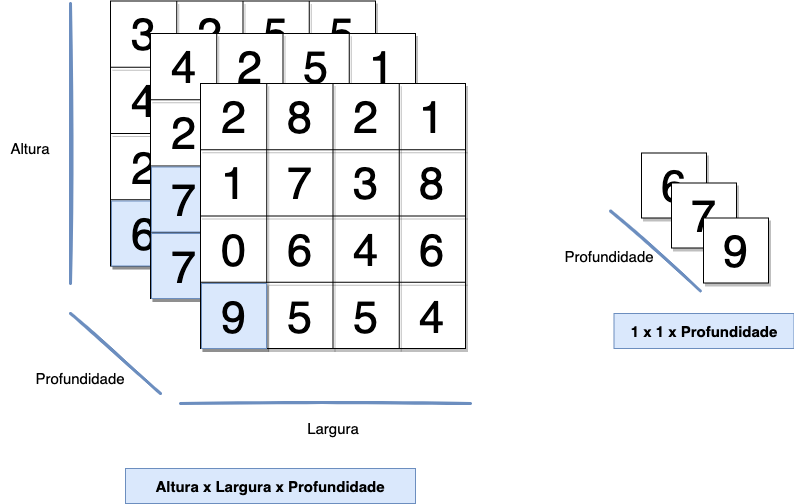
\includegraphics[height=3in]{recursos/imagens/deep/global_max_pooling.png}
    \label{cnn:fig:gmax_pooling}
    
    \caption*{Fonte: do próprio autor.}
\end{figure}

Entretanto, é crucial ressaltar que os métodos convencionais não preservam informações espaciais. Isso se aplica ainda mais aos métodos globais, os quais resumem toda a representação da entrada em um único valor \citep{Christlein2019DeepPooling}. Essa perda de informações espaciais pode ser limitante em algumas tarefas, especialmente em contextos onde a disposição e a relação entre os elementos na entrada têm um papel significativo na análise ou no reconhecimento de padrões.

\subsubsection{\textit{Atrous Spatial Pyramid Pooling}(ASPP)}
\label{cnn:pooling:aspp}
Além da proposta de preservação de escala, embora ainda sem manter a espacialidade, foi introduzido o método \textit{Atrous Spatial Pyramid Pooling} (ASPP) por \cite{Chen2018}. Este tipo de operação de \textit{pooling} está intrinsecamente ligado às segmentações semânticas \citep{Mohan2020} (que serão discutidas no Capítulo \ref{semantic}). A principal vantagem desse algoritmo é a capacidade de capturar objetos e contexto relevantes da imagem em várias escalas distintas. Essa funcionalidade está associada à reamostragem utilizando convoluções com diferentes taxas de dilatação para cada \textit{kernel}, permitindo explorar um mapa de características com múltiplos campos de visão antes mesmo do processo de convolução \citep{Chen2018}. Um exemplo desse módulo pode ser visualizado na Figura \ref{cnn:fig:aspp}.

\begin{figure}[H]
    \centering
    \caption{Exemplo ilustrativo do ASPP.}
    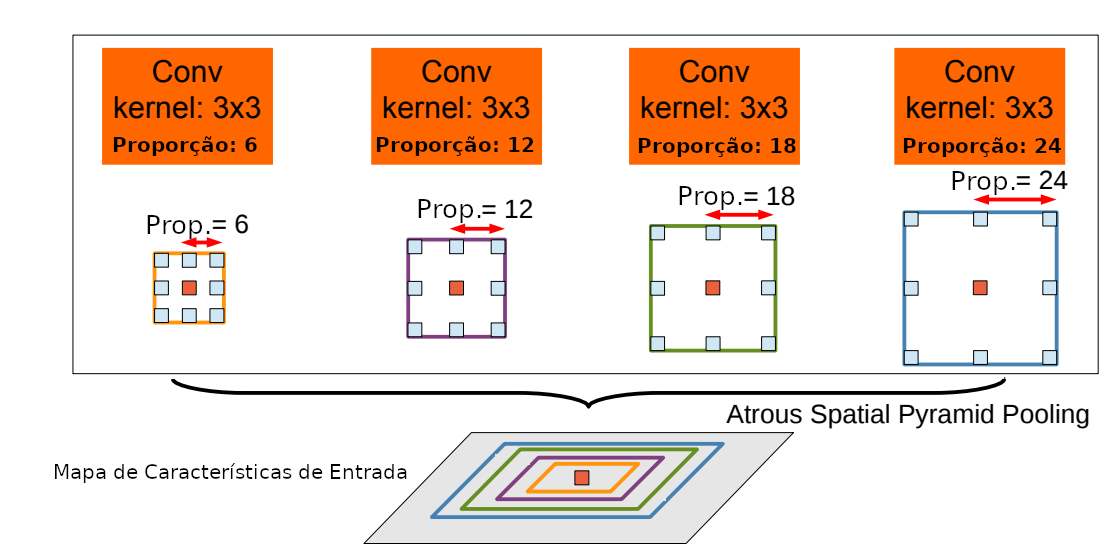
\includegraphics[width=1\textwidth]{recursos/imagens/project/aspp.png}
    \label{cnn:fig:aspp}

    Fonte: Adaptado de \cite{Chen2018}.
\end{figure}

O funcionamento do ASPP, que realiza ajustes no mapa de características para calcular informações em múltiplas escalas, pode ser expresso pela Equação \ref{cnn:eq:pooling:aspp}, proposta por \cite{Chen2018}:

\begin{equation}
    \label{cnn:eq:pooling:aspp}
    y[i] = \sum_{k}x[i + r \cdot k]w [k],
\end{equation}
onde $r$ representa uma taxa de dilatação que determina as \textit{strides} para amostrar o mapa de características de entrada $x$, tendo que para cada \textit{pixel} $i$ na saída $y$ e com o filtro $w$, a convolução dilatada (em inglês, \textit{atrous convolution}) sendo aplicada.

\subsection{\textit{Dropout}}
\label{cnn:dropout}

Dentre as estratégias para mitigar o \textit{overfitting}, citado na Seção \ref{deep:overunder}, destaca-se a técnica de \textit{dropout} \citep{Goodfellow2016}. Esta técnica, embora não seja aplicada durante a fase de testes, consiste no desligamento aleatório de neurônios em camadas ocultas de uma rede CNN. O propósito do \textit{dropout} é reduzir o viés dos neurônios e aumentar a importância dos neurônios restantes.

O processo de \textit{dropout} é ilustrado na Figura \ref{cnn:fig:9}, mostrando apenas as conexões entre os neurônios restantes, no lado direito da Figura \ref{cnn:fig:9}.

\begin{figure}[H]
    \centering
    \caption{Processo de \textit{dropout}.}
    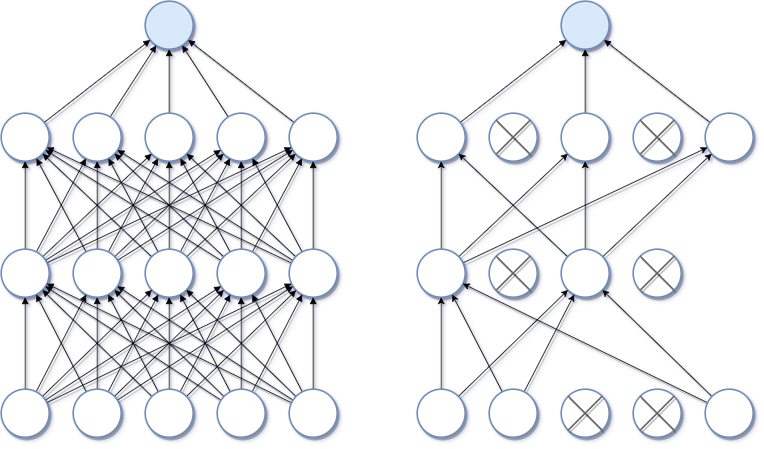
\includegraphics[width=1\linewidth]{recursos/imagens/deep/dropout.png}
    \label{cnn:fig:9}

     Fonte: do próprio autor.
\end{figure}

A técnica de \textit{dropout} é uma estratégia eficaz para regularização em redes neurais, pois ajuda a evitar que a rede se ajuste excessivamente aos dados de treinamento, tornando-a mais capaz de generalizar para dados novos e não vistos durante o treinamento.

\subsection{Camada de Saída}
\label{cnn:output}
Após a composição de várias camadas de convolução, utilizando filtros, e a aplicação de camadas de \textit{pooling}, os modelos de CNN geralmente incluem uma camada de saída. Esta camada é fundamental para a determinação das classes identificadas na imagem. Vale destacar que essa camada não tem um impacto significativo no desempenho em relação ao tempo de convergência do modelo, nem interfere no progresso e evolução do processo de treinamento, sendo que o processo de inferência é muito similar ao usado pelas redes neurais no Capitulo \ref{deep}.

Por fim, para gerar a saída final, é comum utilizar funções de ativação como a Softmax (abordada na Seção \ref{deep:soft}). A aplicação da Softmax permite a identificação da classe de um objeto específico em uma imagem, por exemplo. Essa função de ativação é utilizada para a tarefa de classificação, fornecendo as probabilidades de pertencimento a cada classe no conjunto de dados.

\subsection{Transferência de Aprendizado}
\label{cnn:transfer}

A transferência de aprendizado é uma técnica valiosa no campo da aprendizagem profunda, que sustenta a ideia de usar conhecimento adquirido ao resolver um problema para ajudar a resolver um problema diferente, mas relacionado. Particularmente na aprendizagem profunda, a transferência de aprendizado tem se mostrado benéfica, especialmente, quando se lida com conjuntos de dados com limitações \citep{Pan2010}.

A mais comum estratégia de aplicação da transferência de aprendizado em CNNs é o uso de modelos pré-treinados, onde uma rede treinada em uma tarefa grande e bem definida, como a classificação de imagens em ImageNet \citep{Deng2009ImageNet:Database}, é reutilizada em outra tarefa específica. Isso é feito substituindo as últimas camadas do modelo pré-treinado para se ajustar à tarefa específica e treinando o modelo para ajustar esses novos parâmetros \citep{Yosinski2014HowNetworks}. Com essa mudança, as camadas ou pesos reaproveitados veêm inicialmente de modo \quotes{congelado}, de modo que não há atualização dos erros dessa camada no processo de retropropagação.

Essa abordagem é altamente eficaz, uma vez que durante a fase inicial do treinamento, conhecida como \textit{warmup}, os modelos aprendem características de baixo nível nas camadas iniciais e gradualmente capturam características mais abstratas nas camadas posteriores. A premissa é que as camadas iniciais do modelo extraem recursos genéricos, como bordas e texturas, que são fundamentais para uma ampla variedade de tarefas, enquanto as camadas finais são mais especializadas na tarefa específica para a qual o modelo foi originalmente treinado \citep{Yosinski2014HowNetworks}.

É importante ressaltar que a aplicação da transferência de aprendizado também contribui significativamente para mitigar o \textit{overfitting} \citep{Geron2017Hands-onSystems}. Após a fase de \textit{warmup}, ocorre o gradual \textit{descongelamento} das camadas, iniciando o processo de ajuste fino (ou \textit{fine-tuning}), permitindo que as camadas se adaptem melhor ao problema atual. Quanto mais dados estiverem disponíveis no conjunto, mais camadas ou blocos podem ser descongelados para ajustes finos \citep{Geron2017Hands-onSystems}.

Utilizando transferência de aprendizado, a comunidade pode economizar tempo e recursos computacionais, evitando treinar uma rede complexa do zero para cada nova tarefa. Além disso, modelos pré-treinados podem ajudar a melhorar o desempenho do aprendizado, principalmente quando o conjunto de dados da nova tarefa é pequeno ou semelhante ao conjunto de dados inicial do modelo pré-treinado \citep{Pan2010}.

Apesar dessas vantagens, aplicar transferência de aprendizado em CNNs não é uma tarefa trivial. A seleção e ajuste das camadas para a tarefa pretendida, bem como a seleção das políticas adequadas de otimização e a taxa de aprendizado, são desafios que podem afetar a eficácia da transferência de aprendizado \citep{Yosinski2014HowNetworks}.

Não obstante, a transferência de aprendizado continua sendo uma estratégia amplamente vencedora na atual prática de aprendizagem profunda e sua aplicação está em crescimento contínuo, especialmente em tarefas como análise de sentimentos, detecção de objetos, reconhecimento facial, dentre outros \citep{Pan2010}.

\subsection{Aumento de Dados}
\label{cnn:augment}

A técnica conhecida como aumento de dados, ou \textit{data augmentation} em inglês, é uma estratégia que visa mitigar o \textit{overfitting} e aumentar a robustez do modelo. Essa abordagem consiste em aplicar transformações geométricas e de intensidade nas imagens durante o processo de treinamento, introduzindo variações nas instâncias para enriquecer o conjunto de dados \citep{Geron2017Hands-onSystems}.

A utilização desse método apresenta a vantagem de aumentar a invariância do modelo diante de alterações nas condições de captura das imagens. Por meio dessas transformações, é possível criar diversas variações em termos de escala, posição, cor, luminosidade, saturação e contraste dos objetos, promovendo uma maior capacidade de generalização do modelo. Isso assegura que o reconhecimento das figuras ocorra em diferentes contextos adversos. A Figura \ref{cnn:augment} ilustra exemplos de algumas dessas técnicas de aumento de dados aplicadas a uma imagem.

\begin{figure}[H]
    \centering
    \caption{Exemplo de aumento de dados com transformações geométricas em um exemplo de pimentão.}
    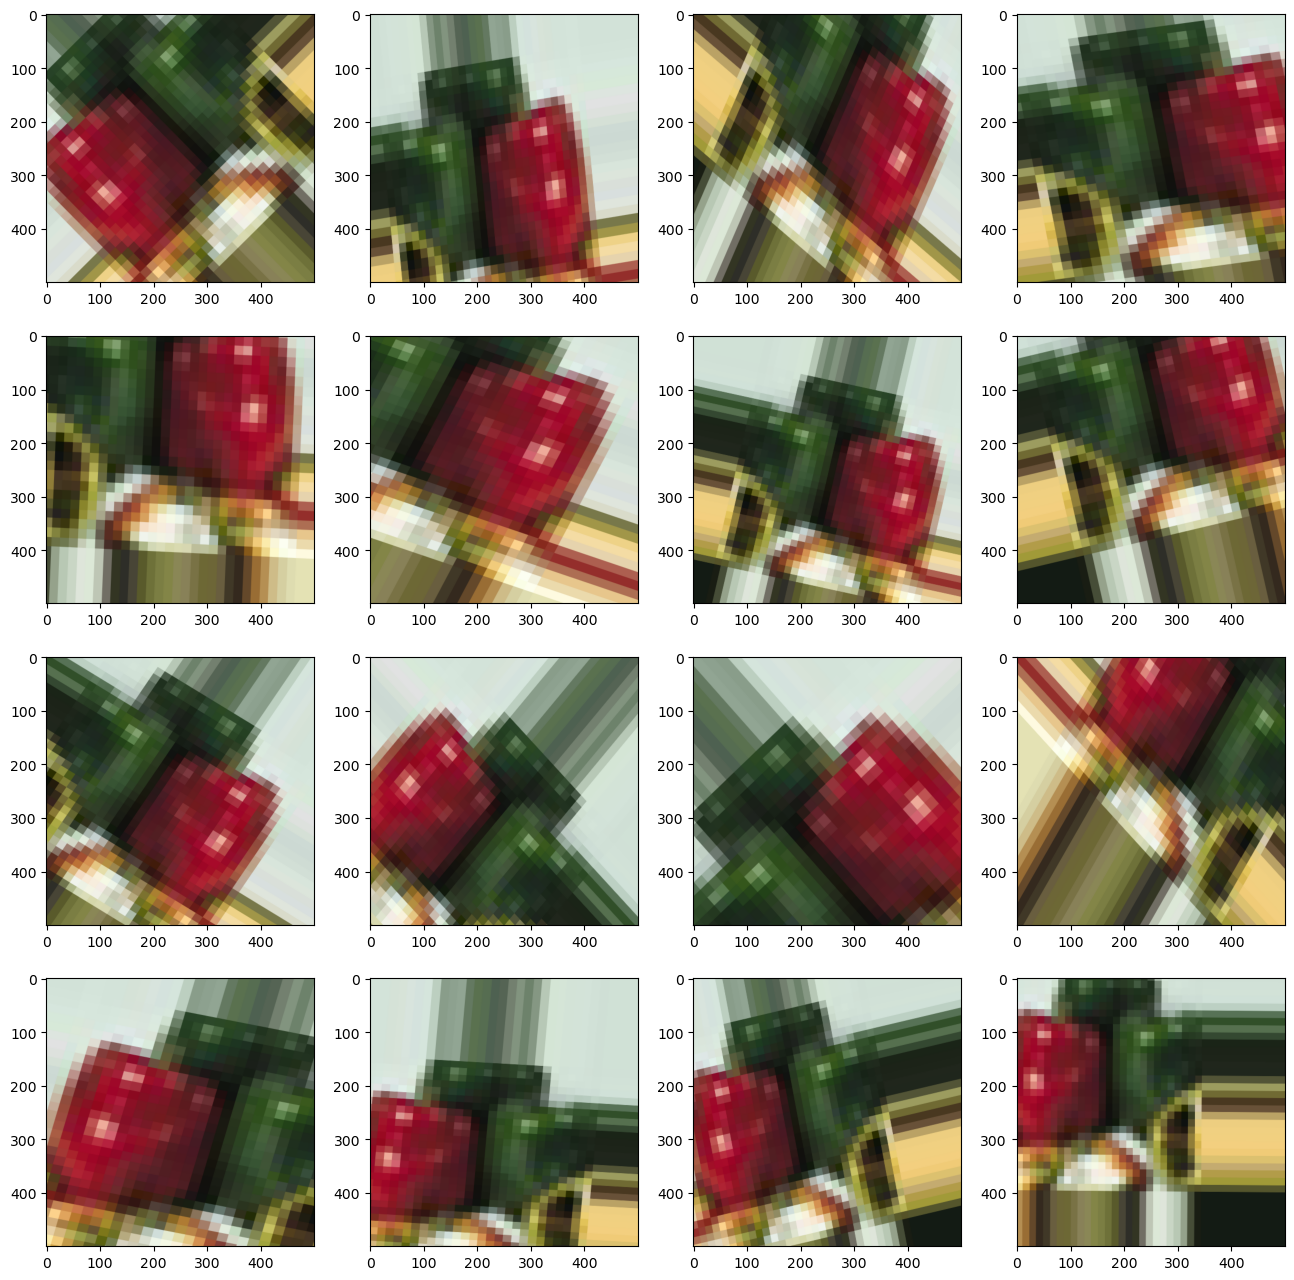
\includegraphics[width=1\linewidth]{recursos/imagens/deep/dataaugmentation.png}
    \label{cnn:fig:augment}

     Fonte: do próprio autor, utilizando o conjunto de dados CIFAR 100\citep{Bossard2014Food-101Forests}.
\end{figure}

Como mencionado anteriormente, é importante destacar que o aumento de dados geralmente envolve o uso de transformações geométricas e de intensidade. As transformações geométricas são responsáveis por aplicar mapeamentos e alterações nos \textit{pixels} das imagens, incluindo rotação, cisalhamento, translação, redimensionamento e outras técnicas comuns usadas em processos de registro de imagens \citep{pedrini2008analise}. Por outro lado, as transformações de intensidade manipulam as cores e os valores dos \textit{pixels}, modificando-os por meio de operações matemáticas como raiz quadrada, potenciação, logaritmos e outras técnicas similares \citep{pedrini2008analise}.

No entanto, é crucial salientar que a seleção das transformações deve ser feita de maneira personalizada para cada problema específico a ser abordado. Isso ocorre porque, além de aumentar a carga computacional, muitas vezes as transformações podem levar à degradação do desempenho do modelo \citep{Carneiro2021EfficientProcessing, Hyttinen2020}. Essas transformações podem modificar o rótulo original do exemplo utilizado ou gerar casos que resultem em falsos positivos ou negativos, como no caso da inversão aplicada ao conjunto de dados MNIST \citep{LeCun2010MNISTDatabase}, ilustrado na Figura \ref{cnn:fig:augment2}, e o uso de \textit{Generative Adversarial Networks} (GANs) em áreas sensíveis, como na medicina.

\begin{figure}[H]
    \centering
    \caption{Exemplo de inversão no conjunto de dados MNIST, em que o dígito \quotes{5} é alterado para \quotes{2}.}
    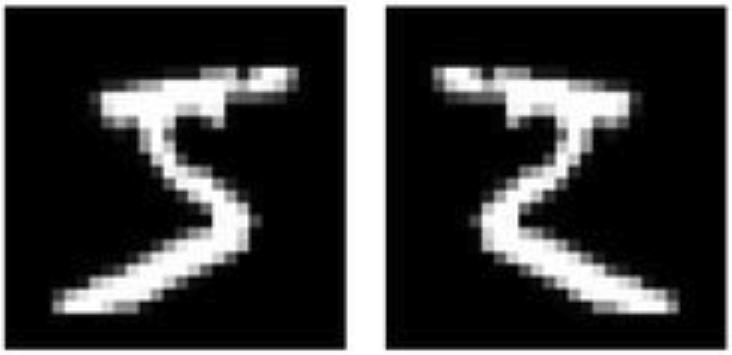
\includegraphics[width=1\linewidth]{recursos/imagens/deep/fivetwo.png}
    \label{cnn:fig:augment2}
    Fonte: do próprio autor, utilizando o conjunto de dados \cite{LeCun2010MNISTDatabase}.
\end{figure}

Por fim, é importante destacar que o processo de aumento de dados geralmente ocorre durante o treinamento do modelo, garantindo que os exemplos utilizados para o aprendizado nunca sejam idênticos, contribuindo para a robustez do modelo. Outra abordagem é aplicar o aumento de dados antes do treinamento, mas essa prática pode resultar em um maior consumo de memória e armazenamento.


\subsection{VGG}
\label{cnn:vgg}

A Rede Neural Convolutiva \textit{Visual Geometry Group} (VGG), desenvolvida pelos pesquisadores do grupo VGG na Universidade de Oxford \citep{Simonyan2015}, tem sido uma das arquiteturas mais influentes no campo da Visão Computacional. A VGG proporcionou avanços significativos no entendimento das redes neurais convolutivas por sua simplicidade arquitetônica e eficiência para lidar com tarefas de aprendizado profundo \citep{Simonyan2015}.

A VGG foi projetada com o objetivo de aumentar a profundidade das redes neurais convolutivas, empregando uma estrutura arquitetônica empilhada de camadas convolutivas pequenas, especificamente filtros de $3 \times 3$, seguidas de camadas \textit{max-pooling} \citep{Simonyan2015}. As camadas convolutivas fazem uso de preenchimento (\textit{padding}) para garantir que a espacialidade seja preservada após cada convolução, antes da redução de tamanho por \textit{max-pooling}. Essa abordagem permitiu que a VGG atingisse profundidades de até 19 camadas \citep{Simonyan2015}.

A maior contribuição da VGG à comunidade de aprendizado de máquina foi a constatação de que a profundidade da rede, ou seja, o número de camadas ocultas, tem grande influência no desempenho do modelo \citep{Simonyan2015}. Essa ideia é refletida na arquitetura homogênea da VGG, que emprega uma pilha de camadas convolutivas para aumentar a profundidade da rede de maneira eficiente, afinal a VGG-16 e 19 possuem cinco blocos de convolução, com pelo menos duas camadas de convolução em cada, e uma camada densa, como representado na Figura \ref{cnn:fig:vgg}.


\begin{figure}[H]
   \caption{Representação de VGGs.}
   \centering
   \label{cnn:fig:vgg}
    \begin{subfigure}[t]{0.8\textwidth}
        \centering
        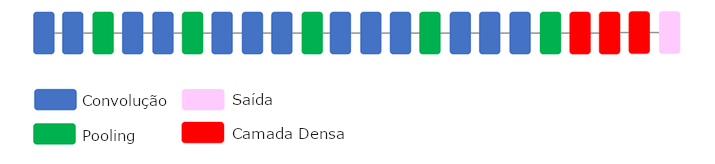
\includegraphics[width=1\linewidth]{recursos/imagens/deep/vgg16.png}
        \caption{VGG-16.}
        \label{cnn:fig:vgg.1}
    \end{subfigure}%
    ~ 

    \begin{subfigure}[t]{0.8\textwidth}
        \centering
        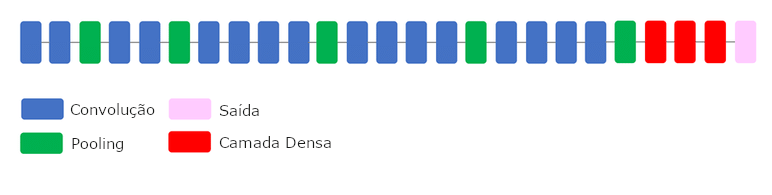
\includegraphics[width=1\linewidth]{recursos/imagens/deep/vgg19.png}
        \caption{VGG-19.}
        \label{cnn:fig:vgg.2}
    \end{subfigure}%
    ~

    Fonte: retirado e adaptado de \cite{Mahdianpari2018VeryImagery}.
\end{figure}

A VGG foi pioneira em demonstrar a utilidade de filtros convolutivos pequenos \citep{Simonyan2015}. Os filtros de $3 \times 3$ podem cobrir a vizinhança imediata de um \textit{pixel} e, quando vários desses filtros são empilhados, a região do campo receptivo pode se expandir e abranger uma maior porção da imagem. Esse processo é similar a aplicar convoluções com filtros maiores, porém, com menos parâmetros. Isso evita o \textit{overfitting} e melhora a capacidade de generalização da rede \citep{Simonyan2015}.

No entanto, a VGG também tem suas limitações. Devido à sua arquitetura profunda, a VGG demanda alto poder computacional e detém grande uso de memória. Além disso, a ausência de camadas totalmente conectadas reduziu a capacidade de modelar dependências de alto nível entre os recursos \citep{Simonyan2015}.

Apesar dessas limitações, a VGG continua sendo amplamente usada na comunidade de aprendizado profundo, principalmente como ponto de partida para a transferência de aprendizado, onde os pesos pré-treinados da VGG são usados como inicialização de outras tarefas de aprendizado. Além disso, a VGG forneceu um ponto de partida sólido para o desenvolvimento de arquiteturas mais profundas e eficientes, como a ResNet \citep{He2016}. Ao introduzir a ideia de profundidade nas redes neurais convolutivas, a VGG marcou um passo importante na evolução das redes de aprendizado profundo.

\subsection{Considerações Finais do Capítulo}
\label{cnn:conclusion}
Neste capítulo é evidenciada a importância das CNNs na abordagem de problemas espaciais, especialmente no domínio de imagens. Foram abordados detalhes sobre como as características são extraídas por meio de filtros e camadas convolucionais (Seção \ref{cnn:conv}), além da forma como as técnicas de \textit{pooling} (Seção \ref{cnn:pooling}) são empregadas para reduzir a dimensionalidade dos dados gerados pelas convoluções. Também se destaca a relevância das camadas de saída (Seção \ref{cnn:output}) na definição das classes presentes na imagem, assim como a aplicação de \textit{dropout} (Seção \ref{cnn:dropout}) para mitigar problemas de \textit{overfitting} (Seção \ref{deep:overunder}), formando assim, arquiteturas profundas, como é o caso das VGGs (Seção \ref{cnn:vgg}).

No entanto, o próximo capítulo se concentrará na segmentação de imagens, uma tarefa mais específica que não requer necessariamente o uso de redes profundas. Muitos métodos podem ser explorados de forma mais artesanal e menos complexa, como será discutido na Seção \ref{segment:segment}.
